\section{Physical Connections and Interfaces}

`v3 sensor boards' means a set of sensors which includs a v3.1 Airsense board, a v3.1 Lightsense board, a Chemsense board, and a alpha sensor.

\begin{figure}[h]
\begin{center}
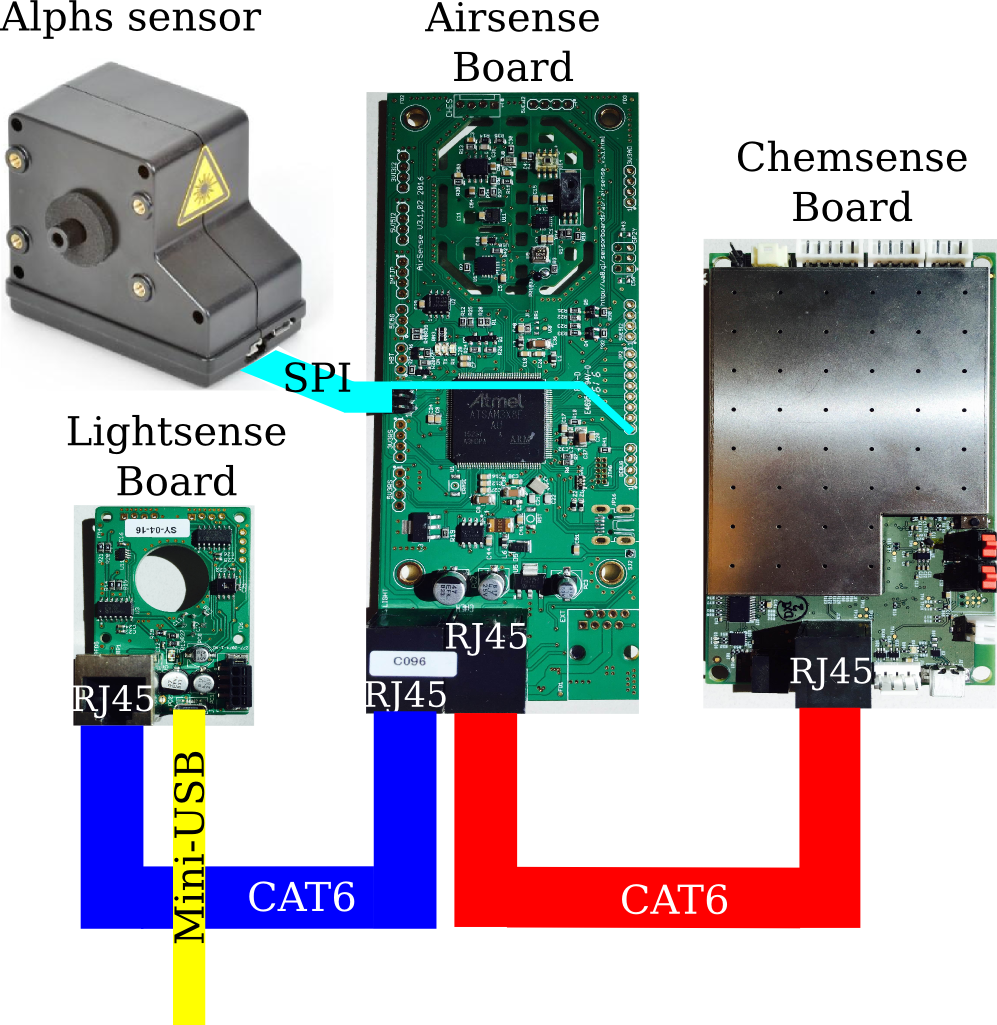
\includegraphics[width=4in]{g4353.png}
\caption{Connections between the sensor boards and the sensor}
\label{fig:physicalConnections}
\end{center}
\end{figure}

Physical connections between sensor boards and sensors are shown in the Figure \ref{fig:physicalConnections}. Airsense board is connected to lightsense board and chemsense board through CAT6 cable. Airsense and lightsense deliver data through I2C communication, and chemsense board delivers data through serial3 communication. All sensor data from airsense, lightsense, and chemsense board are delivered to nodecontroller thourgh USB connect attached on lightsense board. Alpha sensor will be conncted to Airsense board using SPI communication line. Then all the sensor data will be delivered through the USB connect on lighsense board.